% Name: Lever in balance
% Description: A beam on a fulcrum with a load F₁ at distance d₁ on one side and a load half as heavy at twice the distance on the other, so the moments balance, with the support force N.
% Tags: lever, fulcrum, moments, equilibrium, statics

\usetikzlibrary{arrows.meta, patterns}

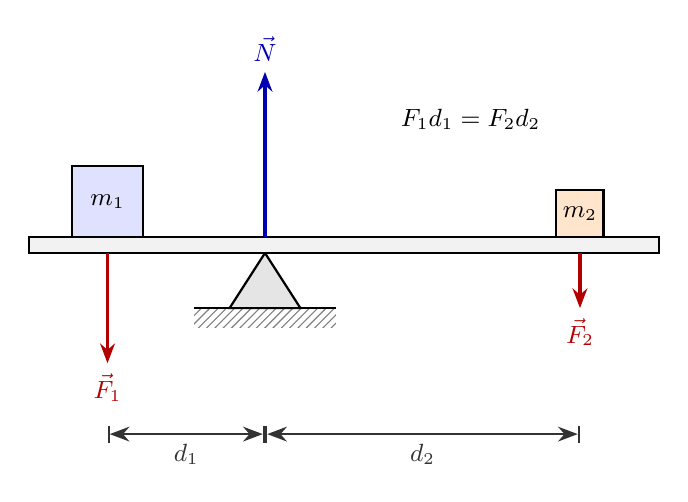
\begin{tikzpicture}[>={Stealth[length=2.5mm]}, force/.style={->, very thick}, every node/.style={font=\small}]
  % Loads 2F at d = 2 and F at d = 4 (arrows 0.7 cm per F): F1 d1 = F2 d2, and N = F1 + F2.
  \fill[pattern=north east lines, pattern color=gray] (-0.9,-1.05) rectangle (0.9,-0.8);
  \draw[thick] (-0.9,-0.8) -- (0.9,-0.8);
  \draw[thick, fill=gray!20] (0,-0.1) -- (0.45,-0.8) -- (-0.45,-0.8) -- cycle;
  \draw[thick, fill=gray!10] (-3,-0.1) rectangle (5,0.1);
  \draw[thick, fill=blue!12] (-2.45,0.1) rectangle (-1.55,1) node[midway] {$m_1$};
  \draw[thick, fill=orange!20] (3.7,0.1) rectangle (4.3,0.7) node[midway] {$m_2$};
  \draw[force, red!70!black] (-2,-0.1) -- ++(0,-1.4) node[below] {$\vec{F}_1$};
  \draw[force, red!70!black] (4,-0.1) -- ++(0,-0.7) node[below] {$\vec{F}_2$};
  \draw[force, blue!70!black] (0,0.1) -- ++(0,2.1) node[above] {$\vec{N}$};
  \draw[|<->|, thick, gray!40!black] (-2,-2.4) -- node[below] {$d_1$} (0,-2.4);
  \draw[|<->|, thick, gray!40!black] (0,-2.4) -- node[below] {$d_2$} (4,-2.4);
  \node[anchor=west] at (1.6,1.6) {$F_1 d_1 = F_2 d_2$};
\end{tikzpicture}
